% Capitolo 4

\chapter{Conclusioni e sviluppi futuri}
\label{Capitolo5}
\lhead{Capitolo 5. \emph{Conclusioni e sviluppi futuri}}

L'architettura e il prototipo sviluppati sono in corso di
implementazione, su scala ridotta, a partire dalle comunità più
strutturate e che fungono già da poli regionali, chiamati
\emph{Nucleos de Formação Continuada, (NFC)}, nuclei di formazione
continua, che sono attualmente dieci, geograficamente ben distribuiti
sul territorio nazionale brasiliano.

Seguendo la filosofia di sviluppo Agile \citep{Agile}, per cui: 

\begin{quote}
  ``\emph{Agile software development is a group of software
    development methods based on iterative and incremental
    development, where requirements and solutions evolve through
    collaboration between self-organizing, cross-functional
    teams.}''\footnote{``Lo sviluppo di software Agile è un insieme di
    metodi basati sullo sviluppo iterativo e incrementale, dove i
    requisiti e le soluzioni evolvono attraverso la collaborazione tra
    team auto-organizzati e multifunzionali.'', tratto da Wikipedia:
    \url{http://en.wikipedia.org/wiki/Agile_software_development}.}
\end{quote}

è importante, in un contesto così ampio e eterogeneo, avere una
struttura generale su cui poter sviluppare codice funzionante, da
poter evolvere e adattare nel tempo.

Il codice prodotto consente una prima implementazione per un progetto
pilota che coinvolga sviluppatori del NPDD e consenta la formazione di
tecnici locali nei NFC, oltre ad ottenere un feedback diretto sull'uso
da parte delle comunità.

Attualmente il codice supporta:
\begin{itemize}
\item autenticazione LDAP (con gestione basica dei gruppi)
\item creazione e upload di contenuti audio, immagini e video
\item distribuzione tramite \emph{git-annex}
\item sincronizzazione degli oggetti sui portali django (ricreando gli
  oggetti relativi ai contenuti distribuiti via \emph{git-annex})
\end{itemize}

Dal punto di vista strutturale la componente più importante è il
sistema di gestione delle identità digitali federate. Pertanto è
essenziale una sperimentazione approfondita della soluzione LDAP
adottata che può comunque essere estesa e integrata ad altri
meccanismi. Per la messaggistica e il VOIP, sarebbe interessante
esplorare le possibilità date dal protocollo XMPP, che si presta per
la facilità con cui può integrarsi in sistemi eterogenei. Ad esempio
l'integrazione tra XMPP e OpenID, per cui, una volta autenticati, si
ricevono le richieste di autorizzazione ad accedere a siti terzi,
tramite messaggi istantanei\footnote{Un'implementazione pubblica di
  questo sistema è disponibile sul sito:
  \url{http://openid.xmpp.za.net/}.}. In questo senso il trio LDAP,
XMPP e OpenID potrebbe offrire una buona struttura per servizi
federati rispettivamente ``desktop'', ``client'' e ``web oriented''.

Per quanto riguardo il prototipo, la parte implementata costituisce un
primo passo, e la prova su campo è un passaggio fondamentale per
testare le reali capacità e i limiti che sussistono. La distribuzione
di file di grandi dimensioni, oltre ai limiti di banda, comporta un
notevole uso di spazio su disco. È necessario quindi imporre dei
limiti, ad esempio, sulle dimensioni massime dei file accettate dal
sistema.

Da implementare o migliorare nelle prossime versioni:
\begin{itemize}
\item trasferimento selettivo dei contenuti/valori basato sull'uso
  statistico o su richiesta
\item sviluppo di in interfaccia di visualizzazione e pubblicazione
  per l'utente finale
\item gestione del DIT dell'LDAP tramite script e/o portale
\end{itemize}

% \begin{figure}[htbp]
%   \centering
%   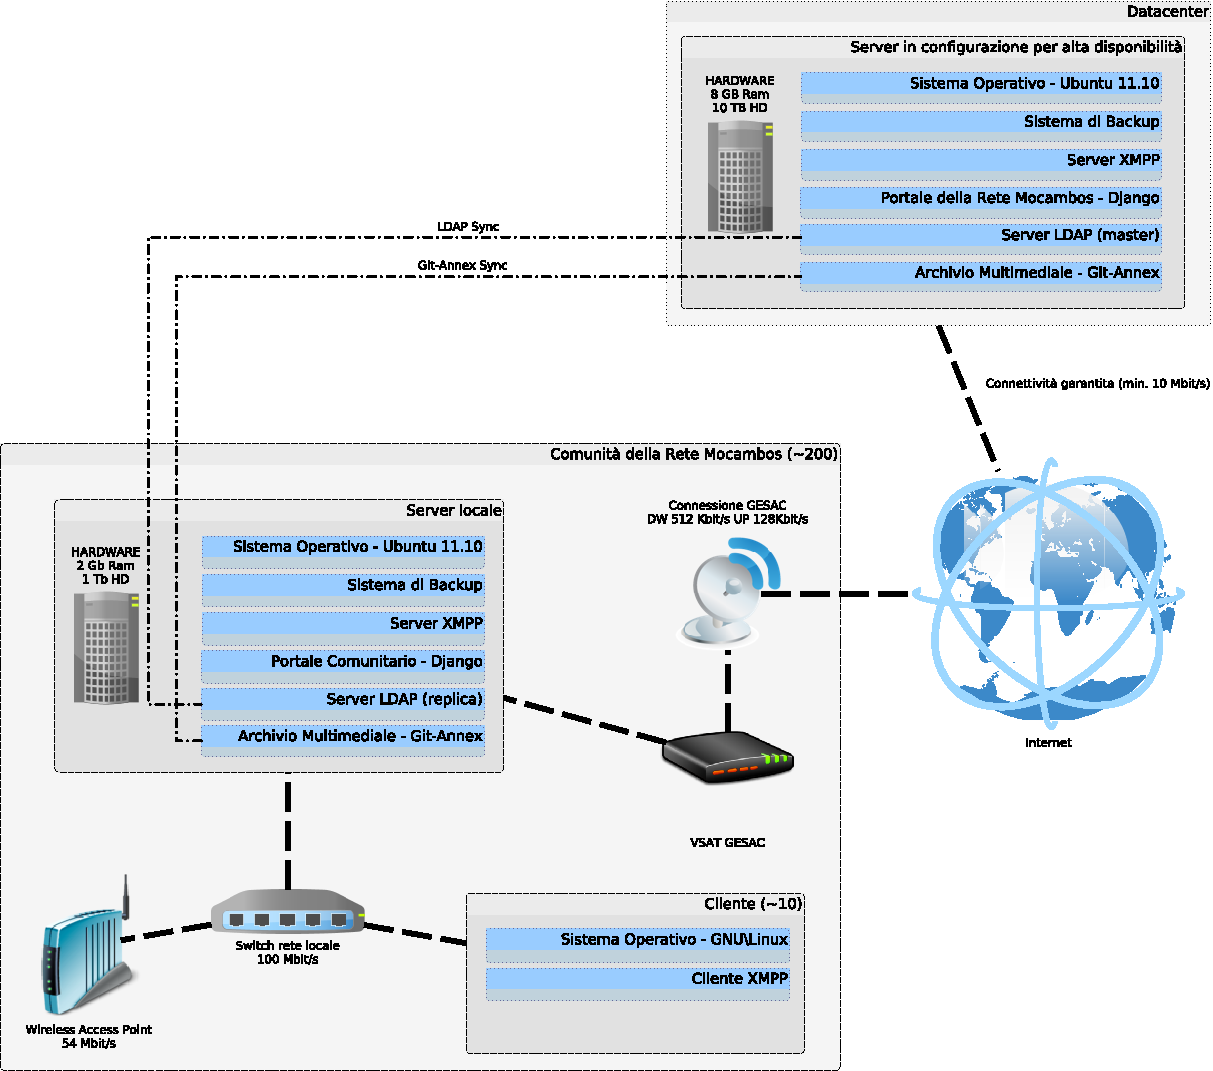
\includegraphics[width=\textwidth]{./Figure/SchemaServer_ReteMocambos-crop.pdf}
%   \rule{35em}{0.5pt}
%   \caption[Schema dell'infrastruttura della RM]{Schema dell'infrastruttura della RM.}
%   \label{fig:SchemaServer_ReteMocambos}
% \end{figure}
